\let\negmedspace\undefined
\let\negthickspace\undefined
\documentclass[journal]{IEEEtran}
\usepackage[a5paper, margin=10mm, onecolumn]{geometry}
%\usepackage{lmodern} % Ensure lmodern is loaded for pdflatex
\usepackage{tfrupee} % Include tfrupee package

\setlength{\headheight}{1cm} % Set the height of the header box
\setlength{\headsep}{0mm}     % Set the distance between the header box and the top of the text
\usepackage{multicol}
\usepackage{gvv-book}
\usepackage{gvv}
\usepackage{cite}
\usepackage{amsmath,amssymb,amsfonts,amsthm}
\usepackage{algorithmic}
\usepackage{graphicx}
\usepackage{textcomp}
\usepackage{xcolor}
\usepackage{txfonts}
\usepackage{listings}
\usepackage{enumitem}
\usepackage{mathtools}
\usepackage{gensymb}
\usepackage{comment}
\usepackage[breaklinks=true]{hyperref}
\usepackage{tkz-euclide} 
\usepackage{pgfplots}
\pgfplotsset{compat=1.18}
\usepackage{listings}
% \usepackage{gvv}                                        
\def\inputGnumericTable{}                                 
\usepackage[latin1]{inputenc}                                
\usepackage{color}                                            
\usepackage{array}                                            
\usepackage{longtable}                                       
\usepackage{calc}                                             
\usepackage{multirow}                                         
\usepackage{hhline}                                           
\usepackage{ifthen}                                           
\usepackage{lscape}
\usepackage{tikz}
% Marks the beginning of the document
\begin{document}
\bibliographystyle{IEEEtran}
\vspace{3cm}

\title{Solving differential equation\\NCERT-12.9.6.3}
\author{EE24BTECH11056 - S.Kavya Anvitha}
\maketitle
%\newpage
\bigskip

\renewcommand{\thefigure}{\theenumi}
\renewcommand{\thetable}{\theenumi}
\textbf{Question:}
\begin{align}
\frac{dy}{dx}+\frac{y}{x} &= x^2
\end{align}
\textbf{Theoretical Solution:}
\begin{align}
    \frac{dy}{dx} + \frac{y}{x} &= x^2 \\
    \text{Integrating Factor: }
    e^{\int \frac{1}{x} \,dx} &= e^{\ln{x}} = x \\
    y \cdot x &= \int x^2 \cdot x \,dx \\
    y \cdot x &= \frac{x^4}{4} + c \\
    \text{Therefore:}\\
    y &= \frac{x^3}{4} + \frac{c}{x}.
\end{align}
Taking C as 1 we get a solution i.e.,
\begin{align}
y &= \frac{x^3}{4} + \frac{1}{x}.
\end{align}
\textbf{Method of finite differences:}
\begin{align}
    \frac{dy}{dx} &= x^2 - \frac{y}{x} \\
    \text{where } \lim_{h \to 0} \frac{y(x+h) - y(x)}{h} &= x^2 - \frac{y}{x} \\
    \end{align}
    \text{Approximaing for small h:}
    \begin{align}
    y_{n+1} - y_n &= h \cdot \brak{x_{n}^2 - \frac{y_n}{x_n}} \\
    \end{align}
    Therefore:
    \begin{align}
    y_{n+1} &= y_n + h \cdot \brak{x_{n}^2 - \frac{y_n}{x_n}} \\
    x_{n+1} &= x_n + h
\end{align}
By initializing the values of x and y and iterating the process several times and plotting
them gives the curve for solution of the differential equation.
\begin{figure}[h!]
   \centering
   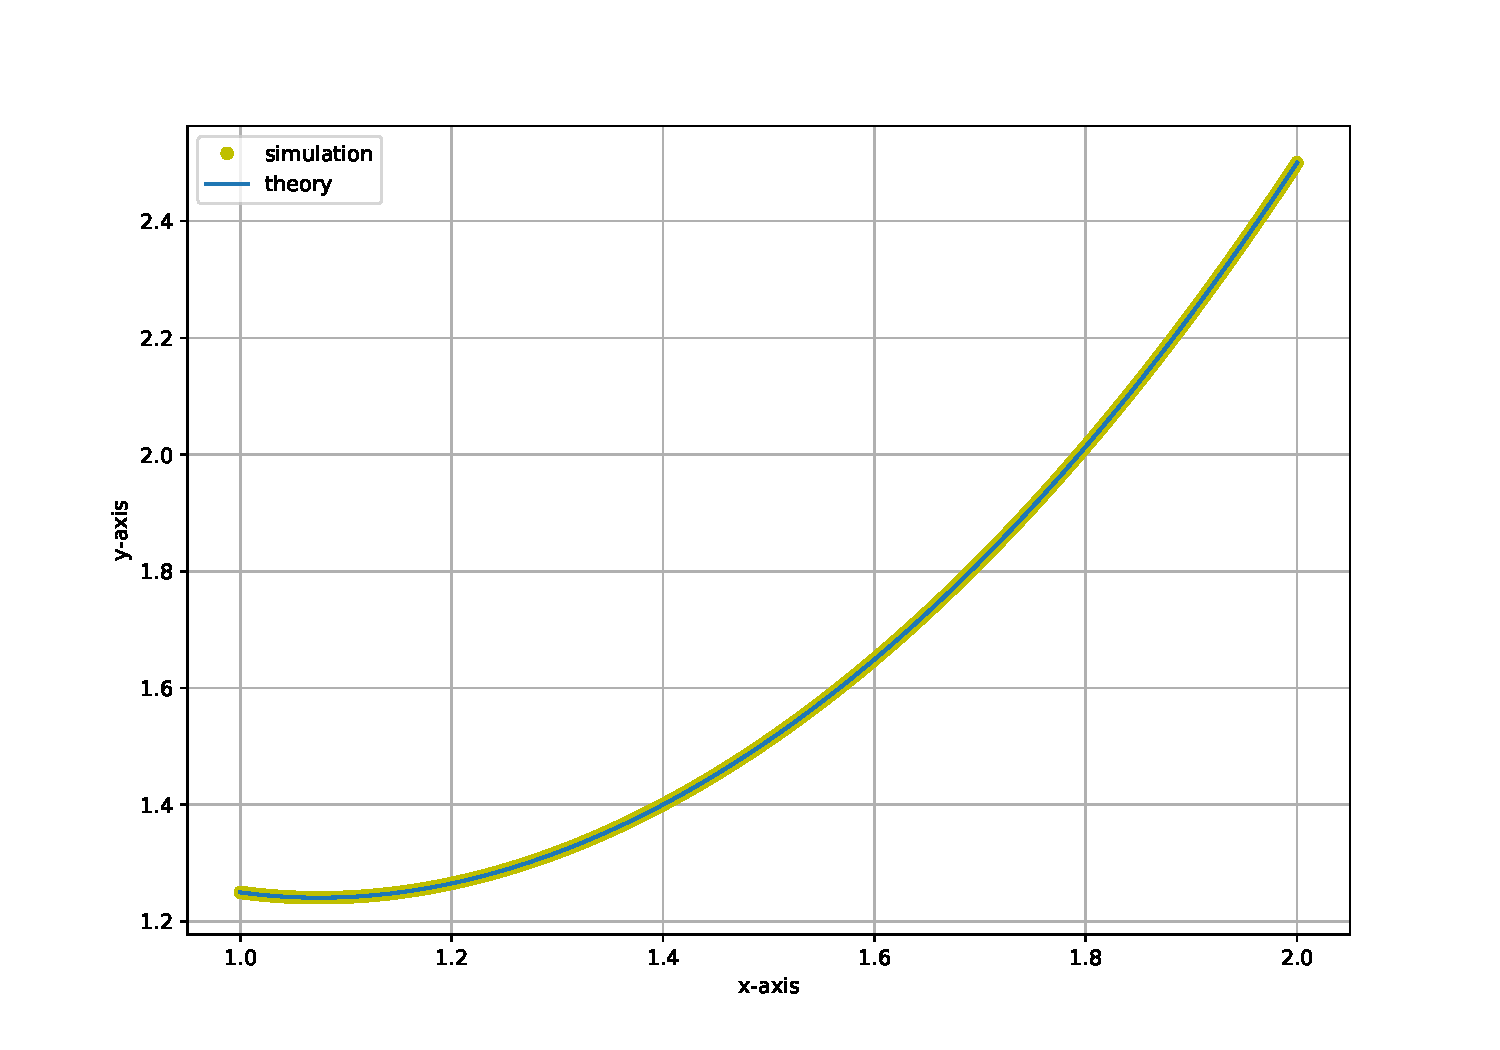
\includegraphics[width=\columnwidth]{figs/combined_plot.pdf}
\end{figure}
\end{document}
